%%%%%%%%%%%%%%%%%%%%%%%%%%%%%%%%%%%%%%%%%%%%%%%%%%%%%%%%%%%%%%%%%
%% ANOTHER LATEX THESIS TEMPLATE.
%% https://github.com/zachscrivena/another-latex-thesis-template
%% This is free and unencumbered software released into the
%% public domain; see <http://unlicense.org> for details.
%%%%%%%%%%%%%%%%%%%%%%%%%%%%%%%%%%%%%%%%%%%%%%%%%%%%%%%%%%%%%%%%%

%%%%%%%%%%%%%%%%%%%%%%%%%%%%%%%%%%%%%%%%%%%%%%%%%%%%%%%%%%%%%%%%%
%% INSTRUCTIONS FOR COMPILING THIS DOCUMENT ("Thesis.tex")
%% TEX ---> DVI ---> PDF.
%%%%%%%%%%%%%%%%%%%%%%%%%%%%%%%%%%%%%%%%%%%%%%%%%%%%%%%%%%%%%%%%%

% Method 1: Use latexmk for fully automated document generation:
%   latexmk -e "$dvipdf='dvipdfm %O -o %D %S'" -pdfdvi "Thesis.tex"
%
% Method 2: Use latex, bibtex, and dvipdfm manually:
%   latex "Thesis.tex"
%   bibtex "Thesis"
%   latex "Thesis.tex" (run multiple times to resolve cross-references)
%   dvipdfm "Thesis.dvi"

\documentclass[oneside,letterpaper,11pt]{report}
% \documentclass[oneside,a4paper,11pt]{report}

%%%%%%%%%%%%%%%%%%%%%%%%%%%%%%%%%%%%%%%%%%%%%%%%%%%%%%%%%%%%%%%%%
%% TYPESETTING OPTIONS.
%%%%%%%%%%%%%%%%%%%%%%%%%%%%%%%%%%%%%%%%%%%%%%%%%%%%%%%%%%%%%%%%%

\newcommand{\TypesetInNonStopMode}{1}
\newcommand{\TypesetInDraftMode}{1}

%%%%%%%%%%%%%%%%%%%%%%%%%%%%%%%%%%%%%%%%%%%%%%%%%%%%%%%%%%%%%%%%%
%% PREAMBLE.
%%%%%%%%%%%%%%%%%%%%%%%%%%%%%%%%%%%%%%%%%%%%%%%%%%%%%%%%%%%%%%%%%

%%%%%%%%%%%%%%%%%%%%%%%%%%%%%%%%%%%%%%%%%%%%%%%%%%%%%%%%%%%%%%%%%
%% ANOTHER LATEX THESIS TEMPLATE.
%% https://github.com/zachscrivena/another-latex-thesis-template
%% This is free and unencumbered software released into the
%% public domain; see <http://unlicense.org> for details.
%%%%%%%%%%%%%%%%%%%%%%%%%%%%%%%%%%%%%%%%%%%%%%%%%%%%%%%%%%%%%%%%%

%%%%%%%%%%%%%%%%%%%%%%%%%%%%%%%%%%%%%%%%%%%%%%%%%%%%%%%%%%%%%%%%%
%% LATEX COMPILATION SETTINGS.
%%%%%%%%%%%%%%%%%%%%%%%%%%%%%%%%%%%%%%%%%%%%%%%%%%%%%%%%%%%%%%%%%

% Run LaTeX in non-stop mode.
\ifnum\TypesetInNonStopMode=1
\nonstopmode
\fi

%%%%%%%%%%%%%%%%%%%%%%%%%%%%%%%%%%%%%%%%%%%%%%%%%%%%%%%%%%%%%%%%%
%% PAGE SIZE AND MARGINS.
%%%%%%%%%%%%%%%%%%%%%%%%%%%%%%%%%%%%%%%%%%%%%%%%%%%%%%%%%%%%%%%%%

% Letter-size (8.5in x 11in) single-sided pages,
% with margins (top,right,bottom,left) = (1,1,1,1.5)in,
% and header 0.25in above the text body.
\usepackage[
total={6in,9in},
top=1in,
left=1.5in,
headsep=0.25in]{geometry}

%%%%%%%%%%%%%%%%%%%%%%%%%%%%%%%%%%%%%%%%%%%%%%%%%%%%%%%%%%%%%%%%%
%% MISCELLANEOUS PACKAGES.
%%%%%%%%%%%%%%%%%%%%%%%%%%%%%%%%%%%%%%%%%%%%%%%%%%%%%%%%%%%%%%%%%

\usepackage[english]{babel} % For language-specific hyphenation.
\usepackage{cite} % Automatically sort and range citations numbers.
\usepackage{environ} % For easy definition of environments.
\usepackage{rotating} % For rotating objects.
\usepackage{framed} % For framed text.

%%%%%%%%%%%%%%%%%%%%%%%%%%%%%%%%%%%%%%%%%%%%%%%%%%%%%%%%%%%%%%%%%
%% PDF OUTPUT.
%%%%%%%%%%%%%%%%%%%%%%%%%%%%%%%%%%%%%%%%%%%%%%%%%%%%%%%%%%%%%%%%%

% PDF metadata and links.
\usepackage[
dvipdfm, % For TEX --> DVI --> PDF.
%pdftex, % For TEX --> PDF.
pdftitle={Insert Thesis Title Here},
pdfauthor={Insert Author Name Here},
pdfsubject={Ph.D. Thesis, University Institute of College, 2014},
pdfcreator={},
pdfproducer={},
pdfkeywords={},
pdfpagemode={},
bookmarks=true,
bookmarksopen=true,
pdfstartview=FitH,
pdfpagelayout=OneColumn,
pdfpagemode=UseOutlines,
pdfstartview=FitH,
hidelinks,
breaklinks]{hyperref}

%%%%%%%%%%%%%%%%%%%%%%%%%%%%%%%%%%%%%%%%%%%%%%%%%%%%%%%%%%%%%%%%%
%% FONTS.
%%%%%%%%%%%%%%%%%%%%%%%%%%%%%%%%%%%%%%%%%%%%%%%%%%%%%%%%%%%%%%%%%

\usepackage[T1]{fontenc}
\usepackage{lmodern} % For Latin Modern fonts.
\usepackage{times} % For Times fonts.

% Sans-serif fonts.
\usepackage[scaled=0.89]{helvet}
\renewcommand{\sffamily}{\usefont{T1}{phv}{m}{n}}
\newcommand{\UseLMSSBoldFont}{\usefont{T1}{lmss}{m}{n}\bfseries}

% Monospace (typewriter) font.
\usepackage[scaled=0.78]{beramono}
\renewcommand{\ttfamily}{\usefont{T1}{fvm}{m}{n}}

%%%%%%%%%%%%%%%%%%%%%%%%%%%%%%%%%%%%%%%%%%%%%%%%%%%%%%%%%%%%%%%%%
%% SECTION HEADINGS.
%%%%%%%%%%%%%%%%%%%%%%%%%%%%%%%%%%%%%%%%%%%%%%%%%%%%%%%%%%%%%%%%%

% Section heading fonts.
\usepackage{sectsty} % For selecting fonts for section headings.
\allsectionsfont{\UseLMSSBoldFont}

% Section numbering depth.
\setcounter{secnumdepth}{10}

%%%%%%%%%%%%%%%%%%%%%%%%%%%%%%%%%%%%%%%%%%%%%%%%%%%%%%%%%%%%%%%%%
%% PARAGRAPHS.
%%%%%%%%%%%%%%%%%%%%%%%%%%%%%%%%%%%%%%%%%%%%%%%%%%%%%%%%%%%%%%%%%

% Line spacing.
\usepackage{setspace}
%\singlespacing
%\onehalfspacing
%\doublespacing
\setstretch{1.6} % custom

% Paragraph indentation:
% Indent first line of all paragraphs (including the first),
% as in IEEE style.
\makeatletter
\let\@afterindentfalse\@afterindenttrue
\makeatother

% Indented blocks.
\newcommand{\IndentBlock}[1]{\noindent\hangafter=0\hangindent=#1\parindent\ignorespaces}
\newcommand{\IndentHanging}{\noindent\hangafter=1\hangindent=\parindent\ignorespaces}

%%%%%%%%%%%%%%%%%%%%%%%%%%%%%%%%%%%%%%%%%%%%%%%%%%%%%%%%%%%%%%%%%
%% HEADERS AND FOOTERS.
%%%%%%%%%%%%%%%%%%%%%%%%%%%%%%%%%%%%%%%%%%%%%%%%%%%%%%%%%%%%%%%%%

% Header.
\newcommand{\HeaderText}{\hfill\footnotesize\sffamily\thepage\hfill}

% Footer.
\ifnum\TypesetInDraftMode=1
\newcommand{\FooterText}{\hfill\footnotesize\sffamily\color{red}{DRAFT}~\Timestamp\hfill}
\fi

\ifnum\TypesetInDraftMode=0
\newcommand{\FooterText}{}
\fi

\makeatletter
\def\ps@plain{%
\def\@oddhead{\HeaderText}%
\def\@evenhead{\HeaderText}%
\def\@oddfoot{\FooterText}%
\def\@evenfoot{\FooterText}}

\makeatletter
\def\ps@empty{%
\def\@oddhead{}%
\def\@evenhead{}%
\def\@oddfoot{\FooterText}%
\def\@evenfoot{\FooterText}}

\pagestyle{plain}

%%%%%%%%%%%%%%%%%%%%%%%%%%%%%%%%%%%%%%%%%%%%%%%%%%%%%%%%%%%%%%%%%
%% FOOTNOTES.
%%%%%%%%%%%%%%%%%%%%%%%%%%%%%%%%%%%%%%%%%%%%%%%%%%%%%%%%%%%%%%%%%

% Blank footnotes.
\newcommand\BlankFootnote[1]{%
\begingroup%
\renewcommand{\thefootnote}{}%
\footnotetext{#1}%
\addtocounter{footnote}{-1}%
\addtocounter{Hfootnote}{-1}%
\endgroup}

%%%%%%%%%%%%%%%%%%%%%%%%%%%%%%%%%%%%%%%%%%%%%%%%%%%%%%%%%%%%%%%%%
%% LISTS.
%%%%%%%%%%%%%%%%%%%%%%%%%%%%%%%%%%%%%%%%%%%%%%%%%%%%%%%%%%%%%%%%%

% Numbered lists in IEEE style.
% (Individual lists can be modified by redefining
% these macros inside the enumerate environment.)
\makeatletter
% 1st level: 1), 2), 3)
\renewcommand{\theenumi}{\arabic{enumi}}
\renewcommand{\labelenumi}{\theenumi)}
% 2nd level: a), b), c)
\renewcommand{\theenumii}{\alph{enumii}}
\renewcommand{\labelenumii}{\theenumii)}
\renewcommand\p@enumii{}
% 3rd level: i), ii), iii)
\renewcommand{\theenumiii}{\roman{enumiii}}
\renewcommand{\labelenumiii}{\theenumiii)}
\renewcommand\p@enumiii{}
% 4th level: A), B), C)
\renewcommand{\theenumiv}{\Alph{enumiv}}
\renewcommand{\labelenumiv}{\theenumiv)}
\renewcommand\p@enumiv{}
\makeatother

% Definition items.
\newcommand{\DefineItem}[1]{%
\IndentBlock{1}#1\nopagebreak
\par\IndentBlock{2}}

%%%%%%%%%%%%%%%%%%%%%%%%%%%%%%%%%%%%%%%%%%%%%%%%%%%%%%%%%%%%%%%%%
%% FIGURES AND TABLES.
%%%%%%%%%%%%%%%%%%%%%%%%%%%%%%%%%%%%%%%%%%%%%%%%%%%%%%%%%%%%%%%%%

\usepackage{graphicx} % To support graphics in EPS format.
\usepackage{multirow} % To support multi-row cells in tables.
\usepackage{booktabs} % For making nice tables.

% Adjust spacing between table rows.
\renewcommand*\arraystretch{1.25}

% Dashed lines in tables.
\usepackage{arydshln}
\def\dashvertical{;{2pt/3pt}}
\def\dashhorizontal{\hdashline[2pt/3pt]}

% Captions for figures and tables.
\newcommand{\CaptionFontSize}{\small}

\makeatletter
\def\@figurestring{figure}
\def\@tablestring{table}
\def\@makecaption#1#2{%
\CaptionFontSize
\ifx\@captype\@figurestring
\vskip1em
\fi
\sbox\@tempboxa{{\sffamily\bfseries{#1.}}\hspace{0.5em}#2}%
\ifdim\wd\@tempboxa>\hsize
{{\sffamily\bfseries{#1.}}\hspace{0.5em}#2}%
\else
\hb@xt@\hsize{\hfil\box\@tempboxa\hfil}%
\fi
\ifx\@captype\@tablestring
\vskip1em
\fi
}
\makeatother

%%%%%%%%%%%%%%%%%%%%%%%%%%%%%%%%%%%%%%%%%%%%%%%%%%%%%%%%%%%%%%%%%
%% COLORS.
%%%%%%%%%%%%%%%%%%%%%%%%%%%%%%%%%%%%%%%%%%%%%%%%%%%%%%%%%%%%%%%%%

\usepackage[usenames]{color} % For colors.
%% \definecolor{MyDarkBlue}{rgb}{0,0.08,0.45}
%% {\color{MyDarkBlue}This text is dark blue}

%%%%%%%%%%%%%%%%%%%%%%%%%%%%%%%%%%%%%%%%%%%%%%%%%%%%%%%%%%%%%%%%%
%% DATE AND TIME.
%%%%%%%%%%%%%%%%%%%%%%%%%%%%%%%%%%%%%%%%%%%%%%%%%%%%%%%%%%%%%%%%%

\usepackage{datetime} % For dates and times.
\renewcommand{\dateseparator}{-}
\settimeformat{xxivtime}

% Timestamp.
\newcommand{\Timestamp}{{\yyyymmdddate\today}~{\currenttime}}

%%%%%%%%%%%%%%%%%%%%%%%%%%%%%%%%%%%%%%%%%%%%%%%%%%%%%%%%%%%%%%%%%
%% COMMENTS, MARKERS, HIDDEN TEXT.
%%%%%%%%%%%%%%%%%%%%%%%%%%%%%%%%%%%%%%%%%%%%%%%%%%%%%%%%%%%%%%%%%

% Comments, markers, hide.
\newcommand{\BoxComment}[1]{{\color{red}\vskip1em\noindent\fbox{\parbox[c]{0.98\columnwidth}{#1}}\vskip1em}}
\newcommand{\Hide}[1]{}

\ifnum\TypesetInDraftMode=1
\newcommand{\TODO}[1]{{\color{red}\fbox{\texttt{TODO}}~#1\color{black}}}
\newcommand{\WIP}{{\BoxComment{~\hfill~\texttt{NOTE: Material below this point is work-in-progress.}~\hfill~}}}
\fi

\ifnum\TypesetInDraftMode=0
\newcommand{\TODO}[1]{}
\newcommand{\WIP}{}
\fi

%%%%%%%%%%%%%%%%%%%%%%%%%%%%%%%%%%%%%%%%%%%%%%%%%%%%%%%%%%%%%%%%%
%% MATHEMATICS.
%%%%%%%%%%%%%%%%%%%%%%%%%%%%%%%%%%%%%%%%%%%%%%%%%%%%%%%%%%%%%%%%%

\usepackage{amsmath,amsfonts,amsbsy,amssymb,amsthm} % AMS packages.

% Indicator function "1[.]" symbol.
% Option 1: Use "\mathbf"
%\newcommand{\one}[1]{{\mathbf{1}\left[#1\right]}}
% Option 2: Use "bbold" package (install "bbold-type1" first)
\DeclareSymbolFont{bbold}{U}{bbold}{m}{n}
\DeclareSymbolFontAlphabet{\mathbbold}{bbold}
\newcommand{\one}[1]{{\mathbbold{1}\left[#1\right]}}
% Option 3: Use "dsfont" package
%\usepackage{dsfont}
%\newcommand{\one}[1]{{\mathds{1}\left[#1\right]}}

% Allow line breaks within math blocks.
\allowdisplaybreaks

% Prevent line breaks within math expressions.
\relpenalty=10000
\binoppenalty=10000
\sloppy

% Theorems (cf. "amsthm.sty").
\newtheoremstyle{MyPlain}%
{0.4em}% space above
{0.4em}% space below
{\itshape}% body font
{}% indent amount
{\sffamily\bfseries}% theorem head font
{.}% punctuation after theorem head
{0.5em}% space after theorem head
{}% theorem head spec

\newtheoremstyle{MyDefinition}%
{0.4em}% space above
{0.4em}% space below
{}% body font
{}% indent amount
{\sffamily\bfseries}% theorem head font
{.}% punctuation after theorem head
{0.5em}% space after theorem head
{}% theorem head spec

\theoremstyle{MyPlain}
\newtheorem{Thm:Theorem}{Theorem}[chapter]
\newtheorem{Thm:Lemma}[Thm:Theorem]{Lemma}
\newtheorem{Thm:Corollary}[Thm:Theorem]{Corollary}
\newtheorem{Thm:Claim}[Thm:Theorem]{Claim}
\newtheorem{Thm:Proposition}[Thm:Theorem]{Proposition}
\newtheorem{Thm:Conjecture}[Thm:Theorem]{Conjecture}

\theoremstyle{MyDefinition}
\newtheorem{Thm:Problem}[Thm:Theorem]{Problem}
\newtheorem{Thm:Definition}[Thm:Theorem]{Definition}
\newtheorem{Thm:Example}[Thm:Theorem]{Example}

\renewenvironment{proof}[1][\proofname]{%
{\par\vskip0.4em\noindent%
\sffamily\bfseries\itshape{#1:}%
\hspace{0.5em}}}%
{\nopagebreak\hspace*{\fill}~\mbox{\rule[0pt]{1.3ex}{1.3ex}}\par}

\newcommand{\qedmarker}{\nopagebreak\hspace*{\fill}~%
\mbox{\rule[0pt]{1.3ex}{1.3ex}}\par}

% Resized "align" environment.
% (may not display correctly in DVI viewer)
\NewEnviron{ResizedAlign}[2]{%
\par\noindent
\resizebox{#1}{!}{
\parbox{#2}{
\begin{align}
\BODY
\end{align}}}\par}

% Resized "align*" environment.
% (may not display correctly in DVI viewer)
\NewEnviron{ResizedAlign*}[2]{%
\par\noindent
\resizebox{#1}{!}{
\parbox{#2}{
\begin{align*}
\BODY
\end{align*}}}\par}

%%%%%%%%%%%%%%%%%%%%%%%%%%%%%%%%%%%%%%%%%%%%%%%%%%%%%%%%%%%%%%%%%
%% CODE.
%%%%%%%%%%%%%%%%%%%%%%%%%%%%%%%%%%%%%%%%%%%%%%%%%%%%%%%%%%%%%%%%%

% Code blocks.
\newcommand{\StartCode}{%
\noindent\ignorespaces%
\begin{framed}
\small\ttfamily
%\def\FrameCommand{{\color{black}{\vrule width 0.5pt\relax\hspace{5pt}}}}%
%\MakeFramed{\advance\hsize-\width\FrameRestore}%
}

\newcommand{\StopCode}{%
\ignorespaces\end{framed}
%\ignorespaces\endMakeFramed%
}

%%%%%%%%%%%%%%%%%%%%%%%%%%%%%%%%%%%%%%%%%%%%%%%%%%%%%%%%%%%%%%%%%
%% TABLE OF CONTENTS (TOC) SETTINGS.
%%%%%%%%%%%%%%%%%%%%%%%%%%%%%%%%%%%%%%%%%%%%%%%%%%%%%%%%%%%%%%%%%

% TOC depth.
\setcounter{tocdepth}{10}

% Suppress entries in the TOC.
\newcommand{\DummyThree}[3]{}

\newcommand{\DisableTOCUpdates}{%
\let\tempaddcontentsline=\addcontentsline
\let\addcontentsline=\DummyThree}

\newcommand{\EnableTOCUpdates}{%
\let\addcontentsline=\tempaddcontentsline}

%%%%%%%%%%%%%%%%%%%%%%%%%%%%%%%%%%%%%%%%%%%%%%%%%%%%%%%%%%%%%%%%%
%% SAMPLE/BLIND TEXT.
%%%%%%%%%%%%%%%%%%%%%%%%%%%%%%%%%%%%%%%%%%%%%%%%%%%%%%%%%%%%%%%%%

\ifnum\TypesetInDraftMode=1
\usepackage{lipsum} % For sample/blind text.
\fi

\ifnum\TypesetInDraftMode=0
\newcommand{\lipsum}[1][]{}
\fi

%%%%%%%%%%%%%%%%%%%%%%%%%%%%%%%%%%%%%%%%%%%%%%%%%%%%%%%%%%%%%%%%%
%% MISCELLANEOUS MACROS.
%%%%%%%%%%%%%%%%%%%%%%%%%%%%%%%%%%%%%%%%%%%%%%%%%%%%%%%%%%%%%%%%%

\DeclareMathOperator*{\argmax}{arg\,max}
\DeclareMathOperator*{\argmin}{arg\,min}
\renewcommand{\binom}[2]{\left(\genfrac{}{}{0pt}{}{#1}{#2}\right)}
\newcommand{\ceil}[1]{{\left\lceil{#1}\right\rceil}}
%\newcommand{\ffrac}[2]{{\nicefrac{#1}{#2}}}
%\newcommand{\fffrac}[2]{{\left.{#1}\middle/{#2}\right.}}
\newcommand{\floor}[1]{{\left\lfloor{#1}\right\rfloor}}
\DeclareMathOperator{\lcm}{lcm}
\newcommand{\ZZ}{{\mathbb{Z}}}


% PDF settings and properties (for "hyperref" package).
\hypersetup{
pdftitle={Insert Thesis Title Here},
pdfauthor={Insert Author Name Here},
pdfsubject={Ph.D. Thesis, University Institute of College, 2014},
pdfcreator={LaTeX},
pdfproducer={},
pdfkeywords={},
pdfpagemode={},
bookmarks=true,
bookmarksopen=true,
pdfstartview=FitH,
pdfpagelayout=OneColumn,
pdfpagemode=UseOutlines,
hidelinks,
breaklinks,
bookmarksnumbered}

%%%%%%%%%%%%%%%%%%%%%%%%%%%%%%%%%%%%%%%%%%%%%%%%%%%%%%%%%%%%%%%%%
%% ACTUAL DOCUMENT.
%%%%%%%%%%%%%%%%%%%%%%%%%%%%%%%%%%%%%%%%%%%%%%%%%%%%%%%%%%%%%%%%%

\begin{document}

% Use Roman numerals (i, ii, iii, etc.) for page numbers.
\pagenumbering{roman}

%%%%%%%%%%%%%%%%%%%%%%%%%%%%%%%%%%%%%%%%%%%%%%%%%%%%%%%%%%%%%%%%%
%% TITLE PAGE.
%%%%%%%%%%%%%%%%%%%%%%%%%%%%%%%%%%%%%%%%%%%%%%%%%%%%%%%%%%%%%%%%%

% No headers or footers on the title page.
\thispagestyle{empty}

\begin{titlepage}
\centering
\setstretch{1.0}
\null
\vspace*{0.25in}
\UseLMSSBoldFont\huge
Insert Thesis Title Here
\\[0.25em]
Use Multiple Lines If Necessary
\\[0.4in]
\normalfont\large
Thesis by
\\[0.25em]
\UseLMSSBoldFont\Large
Insert Author Name Here
\\[0.4in]
\normalfont\normalsize
In Partial Fulfillment of the Requirements
\\[0.5em]
for the Degree of
\\[0.5em]
Doctor of Philosophy
\vfill
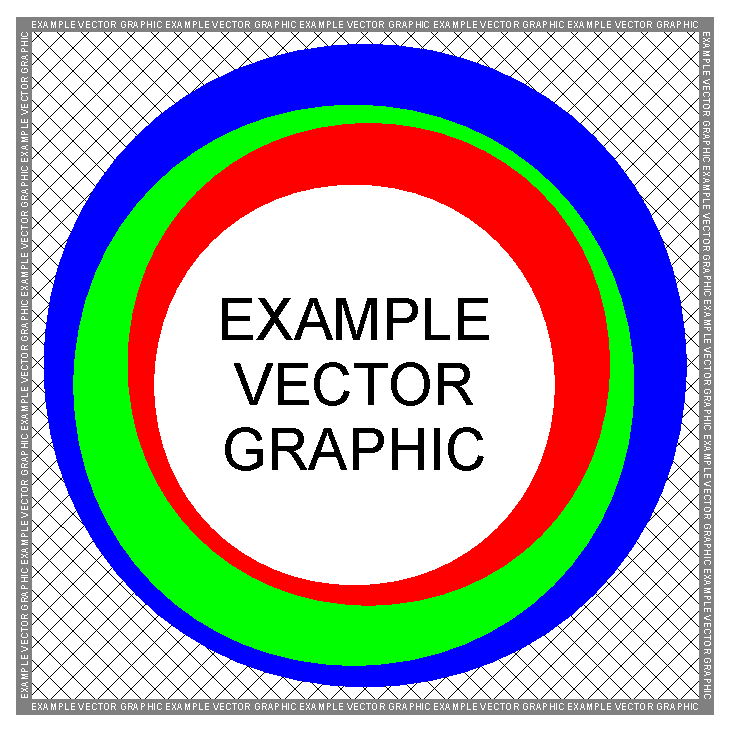
\includegraphics[height=1.8in]
{Figure-SchoolLogo}
\\[0.5em]
University Institute of College
\\[0.5em]
Springfield, New York, USA
\\[1.5em]
2014
\\[0.5em]
(Defended January 7, 2014)
\par
\end{titlepage}

%%%%%%%%%%%%%%%%%%%%%%%%%%%%%%%%%%%%%%%%%%%%%%%%%%%%%%%%%%%%%%%%%
%% COPYRIGHT PAGE.
%%%%%%%%%%%%%%%%%%%%%%%%%%%%%%%%%%%%%%%%%%%%%%%%%%%%%%%%%%%%%%%%%

\pagestyle{plain}
\setcounter{page}{2}

{\centering
\null
\vfill
\raisebox{0.15em}{\scriptsize\sffamily\textcopyright}~2014
\\
Insert Author Name Here
\\
All Rights Reserved
\par}

\clearpage

%%%%%%%%%%%%%%%%%%%%%%%%%%%%%%%%%%%%%%%%%%%%%%%%%%%%%%%%%%%%%%%%%
%% DEDICATION PAGE.
%%%%%%%%%%%%%%%%%%%%%%%%%%%%%%%%%%%%%%%%%%%%%%%%%%%%%%%%%%%%%%%%%

{\centering
\null
\vspace*{1in}
\textit{Insert dedication here}
\par}

\clearpage

%%%%%%%%%%%%%%%%%%%%%%%%%%%%%%%%%%%%%%%%%%%%%%%%%%%%%%%%%%%%%%%%%
%% ACKNOWLEDGMENTS.
%%%%%%%%%%%%%%%%%%%%%%%%%%%%%%%%%%%%%%%%%%%%%%%%%%%%%%%%%%%%%%%%%

\chapter*{Acknowledgments}
\addcontentsline{toc}{chapter}{Acknowledgments}

Insert thesis acknowledgments here.
Thesis acknowledgments typically include research advisers and mentors, thesis committee members, collaborators, and funding sources.

\lipsum[1-2]

\clearpage

%%%%%%%%%%%%%%%%%%%%%%%%%%%%%%%%%%%%%%%%%%%%%%%%%%%%%%%%%%%%%%%%%
%% ABSTRACT.
%%%%%%%%%%%%%%%%%%%%%%%%%%%%%%%%%%%%%%%%%%%%%%%%%%%%%%%%%%%%%%%%%

\chapter*{Abstract}
\addcontentsline{toc}{chapter}{Abstract}

Insert thesis abstract here.
The thesis abstract provides a concise description of the main contributions in the thesis.
Abstracting and indexing services usually include the thesis abstract in the catalog presented to users.
A well-written abstract could improve the chances of your work being discovered and cited by others in the research community.
The abstract should be self-contained (avoid citations and cross references) and should contain only plain text (avoid complicated mathematical expressions).

\lipsum[1-6]

\clearpage

%%%%%%%%%%%%%%%%%%%%%%%%%%%%%%%%%%%%%%%%%%%%%%%%%%%%%%%%%%%%%%%%%
%% TABLE OF CONTENTS (TOC), LISTS OF FIGURES/TABLES/ETC.
%%%%%%%%%%%%%%%%%%%%%%%%%%%%%%%%%%%%%%%%%%%%%%%%%%%%%%%%%%%%%%%%%

\tableofcontents

\listoffigures

\listoftables

\clearpage


% Use Arabic numerals (1, 2, 3, etc.) for page numbers.
\pagenumbering{arabic}

\chapter{Introduction}

Insert thesis introduction here.
\lipsum[1-8]

For more information on this {\LaTeX} thesis template, please visit \url{https://github.com/zachscrivena/another-latex-thesis-template}.


\chapter{Insert Chapter Title Here}
\label{Section:ChapAbbr}

\BlankFootnote{Insert chapter footnote here.
The chapter footnote could include citations to related publications by the author (``The material in this chapter was presented in part in ....'').}

%%%%%%%%%%%%%%%%%%%%%%%%%%%%%%%%%%%%%%%%%%%%%%%%%%%%%%%%%%%%%%%%%
%%%%%%%%%%%%%%%%%%%%%%%%%%%%%%%%%%%%%%%%%%%%%%%%%%%%%%%%%%%%%%%%%
%%%%%%%%%%%%%%%%%%%%%%%%%%%%%%%%%%%%%%%%%%%%%%%%%%%%%%%%%%%%%%%%%

\section{Introduction}
\label{Section:ChapAbbr:Introduction}

Insert chapter introduction here.
\lipsum[1-2]

\mbox{\textit{Related Work:}}
Our work is related to \cite{Examples:Conference01, Examples:Journal01, Examples:Conference02, Examples:Journal02, Examples:Conference03}.
\lipsum[3-4]

\mbox{\textit{Our Contribution:}}
\lipsum[5-6]

Proofs of theorems are deferred to Section~\ref{Section:ChapAbbr:ProofsOfTheorems}.

%%%%%%%%%%%%%%%%%%%%%%%%%%%%%%%%%%%%%%%%%%%%%%%%%%%%%%%%%%%%%%%%%
%%%%%%%%%%%%%%%%%%%%%%%%%%%%%%%%%%%%%%%%%%%%%%%%%%%%%%%%%%%%%%%%%
%%%%%%%%%%%%%%%%%%%%%%%%%%%%%%%%%%%%%%%%%%%%%%%%%%%%%%%%%%%%%%%%%

\section{Some Examples}
\label{Section:ChapAbbr:SomeExamples}

\lipsum[7]

%%%%%%%%%%%%%%%%%%%%%%%%%%%%%%%%%%%%%%%%%%%%%%%%%%%%%%%%%%%%%%%%%
%%%%%%%%%%%%%%%%%%%%%%%%%%%%%%%%%%%%%%%%%%%%%%%%%%%%%%%%%%%%%%%%%
%%%%%%%%%%%%%%%%%%%%%%%%%%%%%%%%%%%%%%%%%%%%%%%%%%%%%%%%%%%%%%%%%

\subsection{Examples of Figures and Tables}
\label{Section:ChapAbbr:SomeExamples:FiguresTables}

%%%%%%%%%%%%%%%%%%%%%%%%%%%%%%%%%%%%%%%%%%%%%%%%%%%%%%%%%%%%%%%%%
% FIGURE: CHAPABBR: FIGURE EXAMPLE A
\begin{figure}
\centering\CaptionFontSize
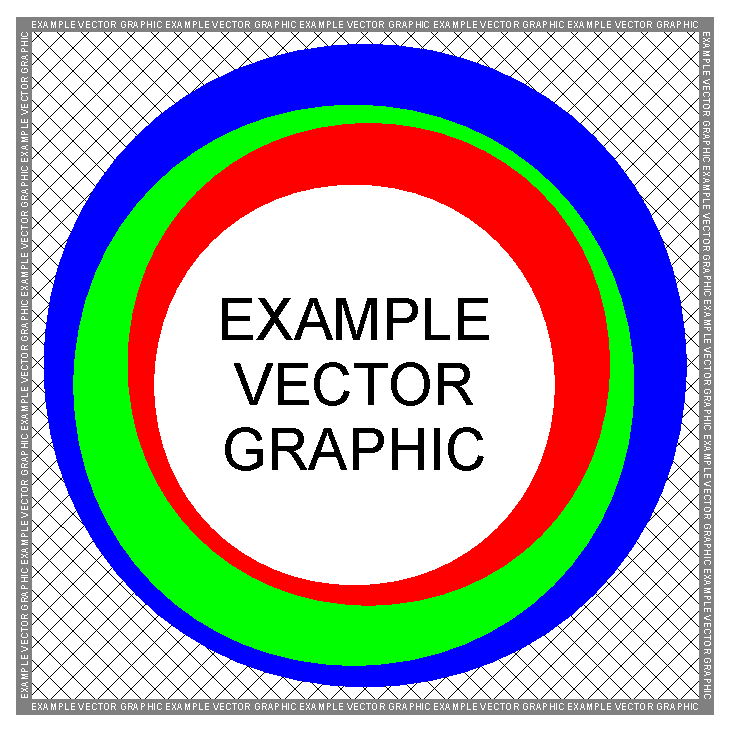
\includegraphics[height=15em]
{Figure-ChapAbbr-FigureExampleA}
\caption[Insert an abbreviated caption here to show in the List of Figures]
{Insert the full caption here for this floating figure.}
\label{Figure:ChapAbbr:FigureExampleA}
\end{figure}
%%%%%%%%%%%%%%%%%%%%%%%%%%%%%%%%%%%%%%%%%%%%%%%%%%%%%%%%%%%%%%%%%

This is a reference to Figure~\ref{Figure:ChapAbbr:FigureExampleA}.
\lipsum[8]

%%%%%%%%%%%%%%%%%%%%%%%%%%%%%%%%%%%%%%%%%%%%%%%%%%%%%%%%%%%%%%%%%
% FIGURE: CHAPABBR: FIGURE EXAMPLE B
\begin{sidewaysfigure*}
\centering\CaptionFontSize
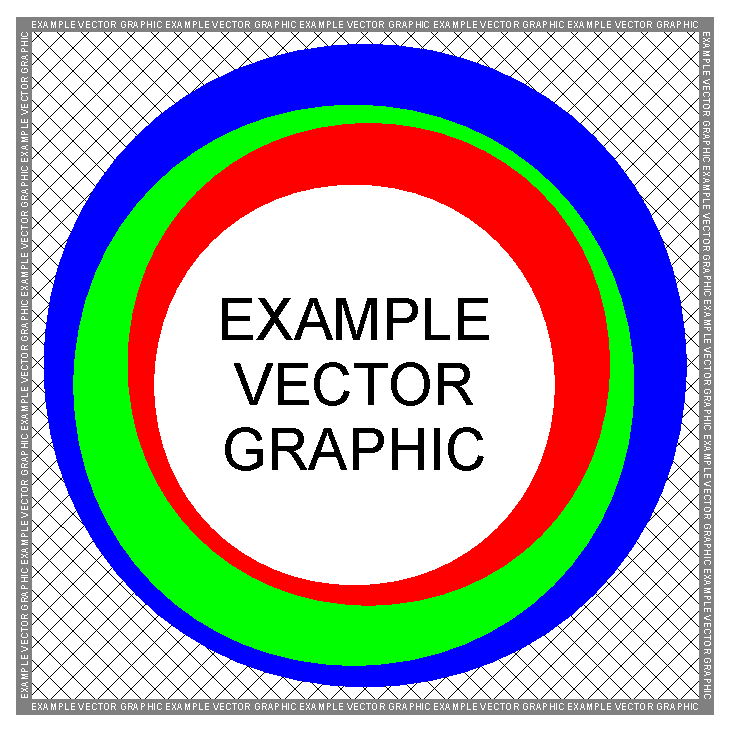
\includegraphics[height=30em]
{Figure-ChapAbbr-FigureExampleB}
\caption[Insert an abbreviated caption here to show in the List of Figures]
{Insert the full caption here for this floating figure.
The caption should provide sufficient context to interpret the figure.
Lorem ipsum dolor sit amet, consectetuer adipiscing elit.
Ut purus elit, vestibulum ut, placerat ac, adipiscing vitae, felis.
Curabitur dictum gravida mauris.}
\label{Figure:ChapAbbr:FigureExampleB}
\end{sidewaysfigure*}
%%%%%%%%%%%%%%%%%%%%%%%%%%%%%%%%%%%%%%%%%%%%%%%%%%%%%%%%%%%%%%%%%

Here we say something about Figure~\ref{Figure:ChapAbbr:FigureExampleB}, and compare it to the earlier Figure~\ref{Figure:ChapAbbr:FigureExampleA}.
\lipsum[9]

%%%%%%%%%%%%%%%%%%%%%%%%%%%%%%%%%%%%%%%%%%%%%%%%%%%%%%%%%%%%%%%%%
% TABLE: CHAPABBR: EXAMPLE A
\begin{table}
\caption[Insert an abbreviated caption here to show in the List of Tables]
{Insert the full caption here for this floating table.}
\label{Table:ChapAbbr:TableExampleA}
\centering\CaptionFontSize
\begin{tabular}{c@{\hspace{1em}}l}
\toprule
Symbol & Definition
\\
\midrule
$\alpha$ & insert definition of $\alpha$ here, $\alpha\geq 1$
\\
$\beta$ & insert definition of $\beta$ here, $\beta\geq 2$
\\
$\gamma$ & insert definition of $\gamma$ here, $\gamma\geq 3$
\\
$\delta$ & insert definition of $\delta$ here, $\delta\geq 4$
\\
\bottomrule
\end{tabular}
\end{table}
%%%%%%%%%%%%%%%%%%%%%%%%%%%%%%%%%%%%%%%%%%%%%%%%%%%%%%%%%%%%%%%%%

We summarize our notation in Table~\ref{Table:ChapAbbr:TableExampleA}.
\lipsum[10]

%%%%%%%%%%%%%%%%%%%%%%%%%%%%%%%%%%%%%%%%%%%%%%%%%%%%%%%%%%%%%%%%%
% TABLE: CHAPABBR: EXAMPLE B
\begin{table}
\caption[Insert an abbreviated caption here to show in the List of Tables]
{Insert the full caption here for this floating table.
The caption should provide sufficient context to interpret the table.
Lorem ipsum dolor sit amet, consectetuer adipiscing elit.
Ut purus elit, vestibulum ut, placerat ac, adipiscing vitae, felis.
Curabitur dictum gravida mauris.}
\label{Table:ChapAbbr:TableExampleB}
\centering\CaptionFontSize
\begin{tabular}{c@{\hspace{1em}}l@{\hspace{1em}}c}
\toprule
Variable & Initial Value & Value at $t=100$
\\
\midrule
$c$ & $0.012$ & $3.456$
\\
$\delta$ & $0.312$ & $1.416$
\\
$\gamma$ & $0.042$ & $3.252$
\\
$h$ & $0.012$ & $3.353$
\\
$c$ & $0.012$ & $4.446$
\\
$\delta$ & $0.015$ & $3.556$
\\
$\gamma$ & $0.612$ & $6.656$
\\
$h$ & $0.072$ & $7.456$
\\
$c$ & $0.018$ & $8.756$
\\
$\delta$ & $0.912$ & $9.456$
\\
$\gamma$ & $0.092$ & $5.956$
\\
$h$ & $0.012$ & $2.326$
\\
\bottomrule
\end{tabular}
\end{table}
%%%%%%%%%%%%%%%%%%%%%%%%%%%%%%%%%%%%%%%%%%%%%%%%%%%%%%%%%%%%%%%%%

Table~\ref{Table:ChapAbbr:TableExampleB} summarizes our simulation results.
\lipsum[11]

%%%%%%%%%%%%%%%%%%%%%%%%%%%%%%%%%%%%%%%%%%%%%%%%%%%%%%%%%%%%%%%%%

\subsection{Examples of Enumerated and Itemized Lists}
\label{Section:ChapAbbr:SomeExamples:Lists}

Here are some citations \cite{Examples:Conference03, Examples:Journal03, Examples:Conference04, Examples:Journal04, Examples:Conference05, Examples:Journal05}.
The following is an enumerated list, or numbered list, with multiple levels:

%%%%%%%%%%%%%%%%%%%%%%%%%%%%%%%%%%%%%%%%%%%%%%%%%%%%%%%%%%%%%%%%%
\begin{enumerate}
\item
\label{Item:ChapAbbr:ItemExampleA}
First level item
\item
First level item
\begin{enumerate}
\item
Second level item
\item
Second level item
\begin{enumerate}
\item
Third level item
\begin{enumerate}
\item
Fourth level item
\item
Fourth level item
\end{enumerate}
\item
Third level item
\end{enumerate}
\item
Second level item
\end{enumerate}
\item
\label{Item:ChapAbbr:ItemExampleB}
First level item
\end{enumerate}
%%%%%%%%%%%%%%%%%%%%%%%%%%%%%%%%%%%%%%%%%%%%%%%%%%%%%%%%%%%%%%%%%

We draw your attention to items \ref{Item:ChapAbbr:ItemExampleA} and \ref{Item:ChapAbbr:ItemExampleB} in particular because they are very important in our study.
The following is an itemized list, or unnumbered list, with multiple levels:

%%%%%%%%%%%%%%%%%%%%%%%%%%%%%%%%%%%%%%%%%%%%%%%%%%%%%%%%%%%%%%%%%
\begin{itemize}
\item
First level item
\item
First level item
\begin{itemize}
\item
Second level item
\item
Second level item
\begin{itemize}
\item
Third level item
\begin{itemize}
\item
Fourth level item
\item
Fourth level item
\end{itemize}
\item
Third level item
\end{itemize}
\item
Second level item
\end{itemize}
\item
First level item
\end{itemize}
%%%%%%%%%%%%%%%%%%%%%%%%%%%%%%%%%%%%%%%%%%%%%%%%%%%%%%%%%%%%%%%%%

%%%%%%%%%%%%%%%%%%%%%%%%%%%%%%%%%%%%%%%%%%%%%%%%%%%%%%%%%%%%%%%%%
%%%%%%%%%%%%%%%%%%%%%%%%%%%%%%%%%%%%%%%%%%%%%%%%%%%%%%%%%%%%%%%%%
%%%%%%%%%%%%%%%%%%%%%%%%%%%%%%%%%%%%%%%%%%%%%%%%%%%%%%%%%%%%%%%%%

\section{Some More Examples}
\label{Section:ChapAbbr:SomeMoreExamples}

According to \cite{IEEEexample:book_typical}, this behavior can be explained this way.
\lipsum[12]

%%%%%%%%%%%%%%%%%%%%%%%%%%%%%%%%%%%%%%%%%%%%%%%%%%%%%%%%%%%%%%%%%
%%%%%%%%%%%%%%%%%%%%%%%%%%%%%%%%%%%%%%%%%%%%%%%%%%%%%%%%%%%%%%%%%
%%%%%%%%%%%%%%%%%%%%%%%%%%%%%%%%%%%%%%%%%%%%%%%%%%%%%%%%%%%%%%%%%

\subsection{Examples of Mathematical Expressions, Definitions, and Theorems}
\label{Section:ChapAbbr:SomeMoreExamples:Math}

We have the following unnumbered mathematical equation:
\[
E=mc^2.
\]
On the other hand, the following is a numbered mathematical inequality:
%%%%%%%%%%%%%%%%%%%%%%%%%%%%%%%%%%%%%%%%%%%%%%%%%%%%%%%%%%%%%%%%%
\begin{align}
x \leq
\frac{\displaystyle\sum_{i=1}^{n} y^2 \cdot \one{y > 1}}
{\displaystyle\int_{-\infty}^{\infty} x^3 \;\text{d}z \cdot
\binom{\alpha}{\beta} \frac{\floor{\frac{a}{b}}}{\ceil{\frac{c}{d}}}}.
\label{Eq:ChapAbbr:EqExample}
\end{align}
%%%%%%%%%%%%%%%%%%%%%%%%%%%%%%%%%%%%%%%%%%%%%%%%%%%%%%%%%%%%%%%%%
Inequality~\eqref{Eq:ChapAbbr:EqExample} will be applied multiple times to prove our theorems, in a manner similar to \cite{IEEEexample:article_typical, IEEEexample:conf_typical}.
We now introduce the following definition:

\begin{Thm:Definition}[Name of Term Being Defined]
This is the definition of the term, along with relevant conditions, trivial cases, exceptions, etc.
\end{Thm:Definition}

We can rewrite the result of \cite[Theorem~2.5]{IEEEexample:conf_typical} in the following convenient form for our problem:

%%%%%%%%%%%%%%%%%%%%%%%%%%%%%%%%%%%%%%%%%%%%%%%%%%%%%%%%%%%%%%%%%
\begin{Thm:Proposition}
For all \mbox{$a,b,c\in\ZZ^+$}, we have
\label{Thm:Proposition:ChapAbbr:PropositionExample}
\[
a^2+b^3\leq c^4.
\]
\end{Thm:Proposition}
%%%%%%%%%%%%%%%%%%%%%%%%%%%%%%%%%%%%%%%%%%%%%%%%%%%%%%%%%%%%%%%%%

Based on our numerical observations, we make the following conjecture about the upper bound:

%%%%%%%%%%%%%%%%%%%%%%%%%%%%%%%%%%%%%%%%%%%%%%%%%%%%%%%%%%%%%%%%%
\begin{Thm:Conjecture}
If \mbox{$x\geq 3$} and \mbox{$0<y<x^2$}, then for all \mbox{$n\in\ZZ^+$},
\[
\sum_{i=1}^{n} x_i
= x_1 + x_2 + \cdots + x_n
\leq T_{\textup{all}}.
\]
\end{Thm:Conjecture}
%%%%%%%%%%%%%%%%%%%%%%%%%%%%%%%%%%%%%%%%%%%%%%%%%%%%%%%%%%%%%%%%%

Here is a lemma that will be quite useful in deriving our results:

%%%%%%%%%%%%%%%%%%%%%%%%%%%%%%%%%%%%%%%%%%%%%%%%%%%%%%%%%%%%%%%%%
\begin{Thm:Lemma}
[Name of Lemma if any]
\label{Thm:Lemma:ChapAbbr:LemmaExampleA}
If \mbox{$x,y,z\in\ZZ^+_0$}, then \mbox{$f(x+y+z) = 1$}.
\end{Thm:Lemma}
%%%%%%%%%%%%%%%%%%%%%%%%%%%%%%%%%%%%%%%%%%%%%%%%%%%%%%%%%%%%%%%%%

Applying Lemma~\ref{Thm:Lemma:ChapAbbr:LemmaExampleA} to \cite[Theorem~4.2]{IEEEexample:book_typical} produces the following theorem:

%%%%%%%%%%%%%%%%%%%%%%%%%%%%%%%%%%%%%%%%%%%%%%%%%%%%%%%%%%%%%%%%%
\begin{Thm:Theorem}
[Name of Theorem if any]
\label{Thm:Theorem:ChapAbbr:TheoremExample}
If \mbox{$x+y\geq z$}, then
\begin{align}
\sum_{i=x}^{y} f(i) \leq z.
\end{align}
\end{Thm:Theorem}
%%%%%%%%%%%%%%%%%%%%%%%%%%%%%%%%%%%%%%%%%%%%%%%%%%%%%%%%%%%%%%%%%

As a special case of Theorem~\ref{Thm:Theorem:ChapAbbr:TheoremExample}, we have the following corollary:

%%%%%%%%%%%%%%%%%%%%%%%%%%%%%%%%%%%%%%%%%%%%%%%%%%%%%%%%%%%%%%%%%
\begin{Thm:Corollary}
If \mbox{$x=4$} and \mbox{$y=z$}, then \mbox{$\sum_{i=x}^{y} f(i) = 5$}.
\end{Thm:Corollary}
%%%%%%%%%%%%%%%%%%%%%%%%%%%%%%%%%%%%%%%%%%%%%%%%%%%%%%%%%%%%%%%%%

\lipsum[13]

%%%%%%%%%%%%%%%%%%%%%%%%%%%%%%%%%%%%%%%%%%%%%%%%%%%%%%%%%%%%%%%%%
%%%%%%%%%%%%%%%%%%%%%%%%%%%%%%%%%%%%%%%%%%%%%%%%%%%%%%%%%%%%%%%%%
%%%%%%%%%%%%%%%%%%%%%%%%%%%%%%%%%%%%%%%%%%%%%%%%%%%%%%%%%%%%%%%%%

\section{Conclusion and Future Work}
\label{Section:ChapAbbr:Conclusion}

\lipsum[14-15]

%%%%%%%%%%%%%%%%%%%%%%%%%%%%%%%%%%%%%%%%%%%%%%%%%%%%%%%%%%%%%%%%%
%%%%%%%%%%%%%%%%%%%%%%%%%%%%%%%%%%%%%%%%%%%%%%%%%%%%%%%%%%%%%%%%%
%%%%%%%%%%%%%%%%%%%%%%%%%%%%%%%%%%%%%%%%%%%%%%%%%%%%%%%%%%%%%%%%%

\section{Proofs of Theorems}
\label{Section:ChapAbbr:ProofsOfTheorems}

\noindent
{\color{red}%
Remember to manually enable and disable table of contents (TOC) updates, using \verb|\EnableTOCUpdates| and \verb|\DisableTOCUpdates|, if you want any subsections, tables, figures, etc., to appear in the table of contents.}

%%%%%%%%%%%%%%%%%%%%%%%%%%%%%%%%%%%%%%%%%%%%%%%%%%%%%%%%%%%%%%%%%

\DisableTOCUpdates

%%%%%%%%%%%%%%%%%%%%%%%%%%%%%%%%%%%%%%%%%%%%%%%%%%%%%%%%%%%%%%%%%

\subsection{Proof of Lemma~\ref{Thm:Lemma:ChapAbbr:LemmaExampleA}}

\lipsum[16-17]
\qedmarker

%%%%%%%%%%%%%%%%%%%%%%%%%%%%%%%%%%%%%%%%%%%%%%%%%%%%%%%%%%%%%%%%%

\subsection{Proof of Theorem~\ref{Thm:Theorem:ChapAbbr:TheoremExample}}

\lipsum[18]

The following lemma will be quite useful in deriving the theorem:

%%%%%%%%%%%%%%%%%%%%%%%%%%%%%%%%%%%%%%%%%%%%%%%%%%%%%%%%%%%%%%%%%
\begin{Thm:Lemma}
\label{Thm:Lemma:ChapAbbr:LemmaExampleB}
If \mbox{$a,b,c\in\ZZ$}, then \mbox{$g(a\cdot b\cdot c) \leq -1$}.
\end{Thm:Lemma}
%%%%%%%%%%%%%%%%%%%%%%%%%%%%%%%%%%%%%%%%%%%%%%%%%%%%%%%%%%%%%%%%%

%%%%%%%%%%%%%%%%%%%%%%%%%%%%%%%%%%%%%%%%%%%%%%%%%%%%%%%%%%%%%%%%%

\begin{proof}
[Proof of Lemma~\ref{Thm:Lemma:ChapAbbr:LemmaExampleB}]
\lipsum[19-20]
\end{proof}

%%%%%%%%%%%%%%%%%%%%%%%%%%%%%%%%%%%%%%%%%%%%%%%%%%%%%%%%%%%%%%%%%

\lipsum[21]
Applying Lemma~\ref{Thm:Lemma:ChapAbbr:LemmaExampleB} yields the following:
%%%%%%%%%%%%%%%%%%%%%%%%%%%%%%%%%%%%%%%%%%%%%%%%%%%%%%%%%%%%%%%%%
\begin{align*}
& A + B + C + D + E + F
+ \alpha + \beta + \gamma + \delta + \Gamma
\\
&\hspace{5em}
\leq
\Omega + \Sigma + \omega + \sigma + \Theta + \theta + \epsilon
+ S + T + U + V + W + X + Y + Z.
\end{align*}
%%%%%%%%%%%%%%%%%%%%%%%%%%%%%%%%%%%%%%%%%%%%%%%%%%%%%%%%%%%%%%%%%
Finally, the desired result is obtained following a simple substitution \mbox{$a=b$}.
\qedmarker

%%%%%%%%%%%%%%%%%%%%%%%%%%%%%%%%%%%%%%%%%%%%%%%%%%%%%%%%%%%%%%%%%

\EnableTOCUpdates

%%%%%%%%%%%%%%%%%%%%%%%%%%%%%%%%%%%%%%%%%%%%%%%%%%%%%%%%%%%%%%%%%
%%%%%%%%%%%%%%%%%%%%%%%%%%%%%%%%%%%%%%%%%%%%%%%%%%%%%%%%%%%%%%%%%
%%%%%%%%%%%%%%%%%%%%%%%%%%%%%%%%%%%%%%%%%%%%%%%%%%%%%%%%%%%%%%%%%

\section{Acknowledgment}
\label{Section:ChapAbbr:Acknowledgment}

Insert chapter acknowledgment here.
\lipsum[22]



\chapter{Summary and Future Work}
\label{Section:Summary}

%%%%%%%%%%%%%%%%%%%%%%%%%%%%%%%%%%%%%%%%%%%%%%%%%%%%%%%%%%%%%%%%%
%%%%%%%%%%%%%%%%%%%%%%%%%%%%%%%%%%%%%%%%%%%%%%%%%%%%%%%%%%%%%%%%%
%%%%%%%%%%%%%%%%%%%%%%%%%%%%%%%%%%%%%%%%%%%%%%%%%%%%%%%%%%%%%%%%%

\section{Summary}
\label{Section:Summary:Summary}

\lipsum[1-6]

%%%%%%%%%%%%%%%%%%%%%%%%%%%%%%%%%%%%%%%%%%%%%%%%%%%%%%%%%%%%%%%%%
%%%%%%%%%%%%%%%%%%%%%%%%%%%%%%%%%%%%%%%%%%%%%%%%%%%%%%%%%%%%%%%%%
%%%%%%%%%%%%%%%%%%%%%%%%%%%%%%%%%%%%%%%%%%%%%%%%%%%%%%%%%%%%%%%%%

\section{Future Work}
\label{Section:Summary:FutureWork}

\lipsum[7-12]


%%%%%%%%%%%%%%%%%%%%%%%%%%%%%%%%%%%%%%%%%%%%%%%%%%%%%%%%%%%%%%%%%
%% BIBLIOGRAPHY.
%%%%%%%%%%%%%%%%%%%%%%%%%%%%%%%%%%%%%%%%%%%%%%%%%%%%%%%%%%%%%%%%%

\clearpage
\phantomsection
\addcontentsline{toc}{chapter}{Bibliography}

\bibliographystyle{IEEEtran} % IEEE bibliographic/citation style.
%\bibliography{IEEEabrv,Thesis}
\bibliography{IEEEfull,Thesis}


\end{document}

%%%%%%%%%%%%%%%%%%%%%%%%%%%%%%%%%%%%%%%%%%%%%%%%%%%%%%%%%%%%%%%%%
%% QUICK REFERENCE.
%%%%%%%%%%%%%%%%%%%%%%%%%%%%%%%%%%%%%%%%%%%%%%%%%%%%%%%%%%%%%%%%%

% Font sizes:
% normalsize, small, footnotesize, scriptsize, tiny
% normalsize, large, Large, LARGE, huge, Huge

% Math delimiter sizes:
% big, Big, bigg, Bigg

% Stacked math expressions:
% \substack{a\\b\\c}
